\subsection{Data Extraction}\label{extraction}
To answer our research questions, we need to mine the repositories of our {\color{blue}fifteen} selected systems to extract information about the \emph{smelliness} of each file at commit level, identifying whether the file contains a code smell or not. In addition, we need to know for each commit, if the commit introduces a bug, fixes a bug{\color{blue}, or introduces a vulnerability,} or just modifies the file in a way that a code smell is removed or added. Figure~\ref{process} provides an overview of our approach {\color{blue}to answer RQ1 and RQ2, Figure~\ref{process2} to answer RQ3 and RQ4, and Figure~\ref{process3} to answer RQ5}. We describe each step in our data extraction approach below. We have implemented all the steps of our approach into a framework available on Github\footnote{https://github.com/DavidJohannesWall/smells\_project}.

\begin{figure*}[t]
\captionsetup{font=small}
\centering%
	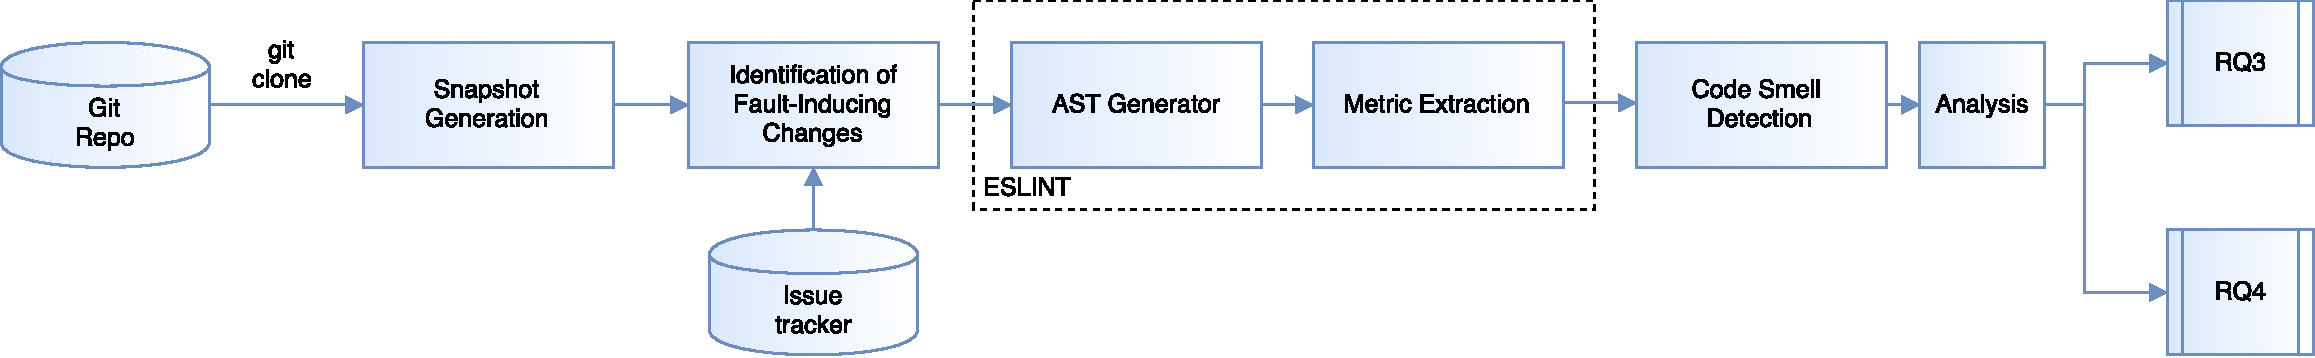
\includegraphics[scale=0.45]{pdfs/total.pdf}
	\caption{Overview of our approach to answer RQ1 and RQ2.}
\label{process}
\vspace{-15pt}
\end{figure*}

\begin{figure*}[t]
	\captionsetup{font=small}
	\centering%
	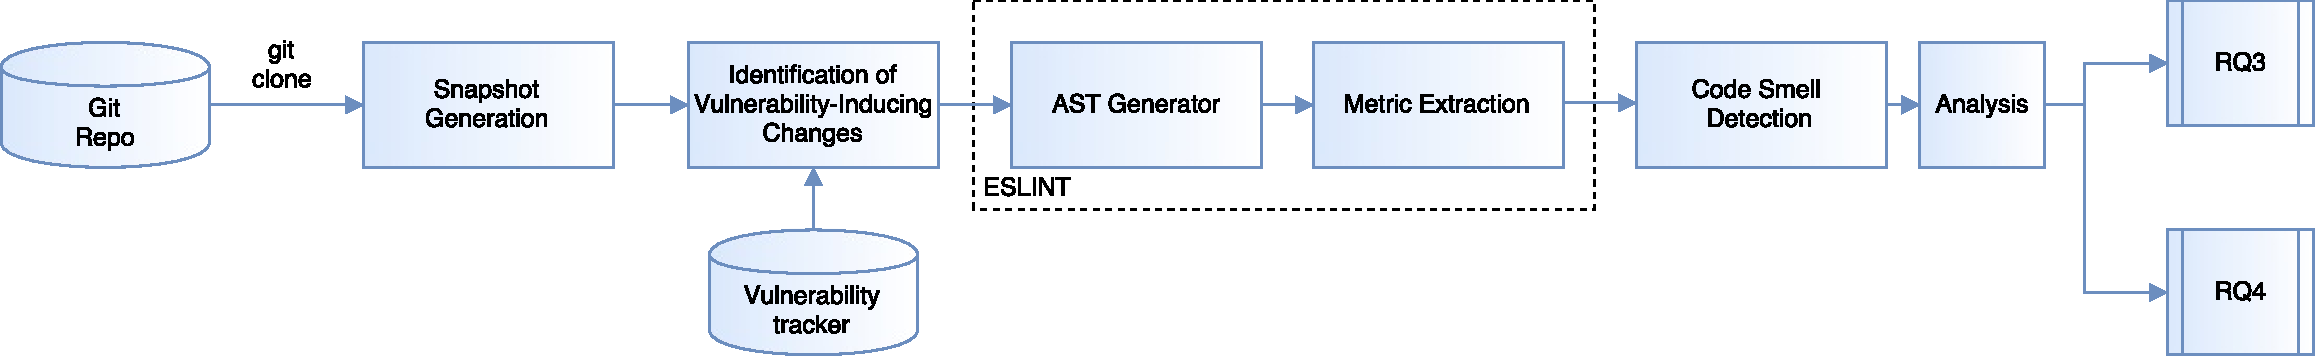
\includegraphics[scale=0.45]{pdfs/total2.pdf}
	\caption{Overview of our approach to answer RQ3 and RQ4.}
	\label{process2}
	\vspace{-15pt}
\end{figure*}

\begin{figure*}[t]
	\captionsetup{font=small}
	\centering%
	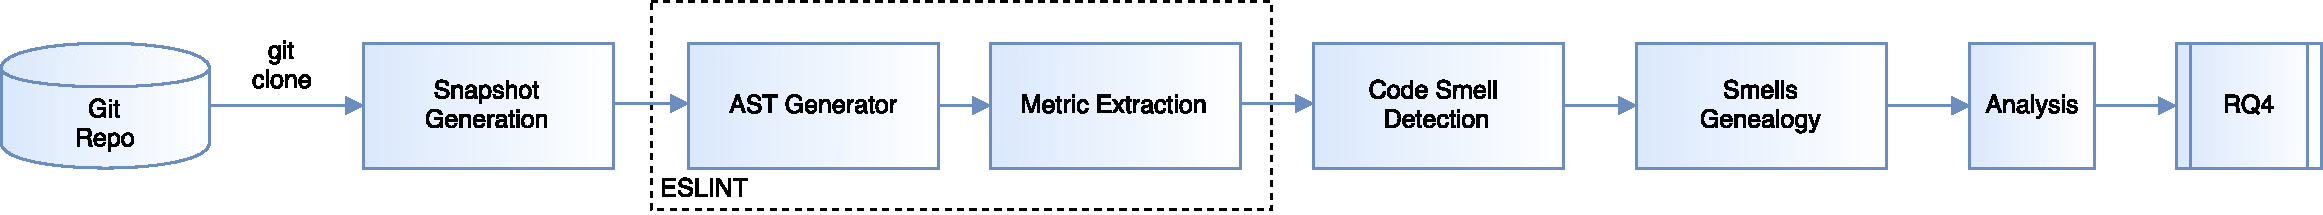
\includegraphics[scale=0.45]{pdfs/total3.pdf}
	\caption{Overview of our approach to answer RQ5.}
	\label{process3}
	\vspace{-15pt}
\end{figure*}

\mytitle{Snapshot Generation} Since all the five studied systems are hosted on Github, at the first step, the framework performs a \texttt{git clone} to get a copy of a system's repository locally. It then generates the list of all the commits and uses it to create snapshots of the system that would be used to perform analysis at commits level.

\mytitle{Identification of Fault-Inducing Changes} Our studied systems use Github as their issue tracker and we use Github APIs to get the list of all the resolved issues on the systems. We leverage the SZZ algorithm~\cite{sliwerski2005changes} to detect changes that introduced faults. We first identify fault-fixing commits using the heuristic proposed by Fischer et al.~\cite{fischer2003populating}, which consists in using regular expressions to detect bug IDs from the studied commit messages. Next, we extract the modified files of each fault-fixing commit through the following Git command:\\

\texttt{git log [commit-id] -n 1 {-{}-}name-status}\\

\noindent
We only take modified JavaScript files into account. Given each file $F$ in a commit $C$, we extract $C$'s parent commit $C'$. Then, we use Git's \texttt{diff} command to extract $F$'s deleted lines. We apply Git's \texttt{blame} command to identify commits that introduced these deleted lines, noted as the ``candidate faulty changes''. We eliminate the commits that only changed blank and comment lines. Then, we filter the commits that were submitted after their corresponding bugs' creation date. {\color{blue}Considering the file $F$ in a fault-fixing commit and its commit that introduced faults, we use again Git's \texttt{diff} command to extract $F$'s changes between both commits, in order to retrieve the ``candidate fault lines'' (useful for our line grain analysis). For the next step, we use UglifyJS\footnote{https://github.com/mishoo/UglifyJS} to get an $F$'s Abstract Syntax Tree (AST) that gives the dependencies of all $F$'s variables, objects and functions (which means their declaration and use lines). We then match $F$'s dependencies with the ``candidate fault lines'' to extend them: given an $F$'s element (variable, object, or function), if one of its declaration or use lines is found into the ``candidate fault lines'', then we add these declaration and use lines to the ``candidate fault lines''. We finally obtain the ``extended candidate fault lines'' (usefull for our line grain analysis including dependencies).

\mytitle{Identification of Vulnerability-Inducing Changes} We use Snyk\footnote{https://snyk.io/test} as our vulnerability tracker. We passe each commit of each project through Snyk which gives us the presence and characteristics (vulnerable module, vulnerability's title, how it is introduced) of commit's vulnerabilities, if they exist or if they are listed by Snyk. Given two vulnerabilities, we consider they are the same if they have the same characteristics, which means the same title, vulnerable modules, and modules through which they were introduced. Given a vulnerability $V$, we only keep the first commit $C$ that introduced for the first time $V$. Then, similarly to the identification of fault-inducing changes, we only take $C$'s modified JavaScript files into account (our ``candidate vulnerability changes''), and for each of those files, we take the last commit before $C$ that modified significantly those files. Given $C$, let's name $F$ one of the $C$'s modified JavaScript file, and $C'$ the last commit before $C$ that modified $F$. The next step is to use Git's \texttt{diff} command to extract $F$'s changes between both commit $C$ and $C'$, in order to retrieve the ``candidate vulnerability lines'' (useful for our line grain analysis), and then to use UglifyJS to keep dependencies in account and get the ``extended candidate vulnerability lines'' (usefull for our line grain analysis including dependencies).
}

\mytitle{AST Generation and Metric Extraction} To automatically detect code smells in the source code, we first extract the Abstract Syntax Tree from the code. AST are being used to parse a source code and generate a tree structure that can be traversed and analyzed programmatically. ASTs are widely used by researchers to analyze the structure of the source code \cite{neamtiu2005understanding, baxter1998clone, pfenning1988higher}.
We used ESLint\footnote{http://eslint.org/} which is a popular and open source lint utility for JavaScript as the core of our framework. Linting tools are widely used in programming to flag the potential non-portable parts of the code by statically analyzing them. ESLint is being used in production in many companies like Facebook, Paypal, Airbnb, etc. ESLint uses espree\footnote{https://github.com/eslint/espree} internally to parse JavaScript source codes and extracts Abstract Source Trees based on the specs\footnote{https://github.com/estree/estree}. ESLint itself provides an extensible environment for developers to develop their own plugins to extract custom information from the source code. We developed our own plugins and modified ESLint built-in plugins to traverse the source tree generated by ESLint to extract and store the information related to our set of code smells described in section \ref{sec:background}. Table~\ref{smellmetric} summarizes all the metrics our framework reports for each type of code smell.

{\color{blue}
\mytitle{Smells Genealogy} Thanks to our previous extraction methods, we easily get, for each Javascript file of a project, the history of the commits that modified those files. Given the history $H$ of a JavaScript file $F$, we identifiy and track $F$'s smells through each commit of $H$. Given two consecutive commits $C1$ and $C2$ of $H$: if one smell appears in $C2$ (and not in $C1$), we consider it as a new smell and keep its date of creation ($C2$'s date); if one smell disappears in $C2$ (and was present in $C1$), we consider it was killed, and keep its date of destruction ($C2$'s date). If a smell if never killed (present in the last commit of $H$), we consider its presence until the last project's commit. To measure the similarity degree between two smells, they first need to be from the same smell type, and then we use SequenceMatcher\footnote{https://docs.python.org/2/library/difflib.html} from difflib (a Python library) that gives us a number between 0 and 1 as a similarity degree (1: both smells are the same; 0: they are totally different). We consider two smells as the same if they are from the same smell type (among the 12 studied), and if their similarity degree is greater than 0.7. If one smell of $C1$ gets a similarity degree greater than 0.7 with two smells of $C2$, we keep the maximum in account. We tried our survival analysis of smells with different thresholds of similarity degree (0.8 and 0.9), but we observe no significant difference with the use of 0.7 threshold.
}

\begin{table*}[!htbp]
\scriptsize
\centering
\caption{Metrics computed for each type of code smell.}
\label{smellmetric}
\begin{tabular}{l|l|l}
\hline
Smell Type                           & Type    & Metric                                                                                                  \\ \hline
Lengthy Lines                        & Number  & The number of characters per line considering the exceptions described in section \ref{sec:background}. \\ \hline
Chained Methods                      & Number  & The number chained methods in each chaining pattern.                                               \\ \hline
Long Parameter List                  & Number  & The number of parameters of each function in source code.                                               \\ \hline
Nested Callbacks                     & Number  & The number of nested functions present in the implementation of each function.                          \\ \hline
Variable Re-assign                   & Boolean & The uniqueness of variables in same scope.                                                              \\ \hline
Assignment in Conditional Statements & Boolean & The presence of assignment operator in conditional statements.                                          \\ \hline
Complex code                         & Number  & The cylcomatic complexity value of each function defined in the source code.                            \\ \hline
Extra Bind                           & Boolean & Whether a function is explicitly bound to a context while not using the context.                        \\ \hline
This Assign                          & Boolean & Whether \texttt{this} is assigned to another variable in a function.                                    \\ \hline
Long Methods                         & Number  & The number of statements in each function.                                                              \\ \hline
Complex Switch Case                  & Number  & The number of case statements in each switch-case block in the source code.                             \\ \hline
Depth                                & Number  & The maximum number of nested blocks in each function.                                                   \\ \hline
\end{tabular}
\vspace{-15pt}
\end{table*}

\mytitle{Code Smell Detection} Among of 12 metric values reported by our framework, 4 are boolean. The boolean metrics concern \emph{This Assign}, \emph{Extra Bind}, \emph{Assignment in Conditional Statements}, and \emph{Variable Re-assign} smells. The 8 remaining metrics are integers. To identify code smells using the metric values provided by our framework, we follow the same approach as previous works~\cite{marinescu2004detection, mazinanian2016migrating}, defining threshold values above which files should be considered as having the code smell. We define the thresholds relative to the systems using Box-plot analysis. We chose to define threshold values relative to the projects because design rules and programming styles can vary from one project to another, and hence it is important to compare the characteristics of files in the context of the project. For each system, we obtain the threshold values as follows. We examined the distribution of the metrics and observed a big gap around the first 70\% of the data and the top 10\%. Hence, we decided to consider files with metric values in the top 10\% as containing the code smell. For files that contain multiple functions, we aggregated the metric values reported for each functions using the maximum to obtain a single value characterizing the file. %of the metric values reported for each function contained in the file to obtain a metric value characterizing the file.

%aformentioned In order to convert those numeric values into boolean which indicate the presence of a type of smell, we used a statistical approach to define the threshold . Since the culture, style guide and design rules could be different from a project to another, we defined the threshold specifically for each project in our case study.
%
%To define the threshold, we first removed the top 1\% of the data to remove extreme cases. By looking at the distribution of the numeric values of extracted metrics, for most of the metrics we saw there is a big gap around the first 70\% of the data and the top 10\%. So we considered the top 10\% of each metric as smelly codes. To analyze the sensitivity of the threshold to the result, we rerun our analysis with the threshold values of top 20\% and top 30\% as well and we observed no significant difference.
%Also as files could contain multiple functions and so multiple smelly parts, our framework could extract multiple values for each file for each numeric metric. To reduce this list of values to a single number, we get the maximum value of the list and associated that with the file.
%
%\section{Code Smells}\label{smells}
%Code smells are the results of bad design choices. They are referred to the structural characteristics in software code which could make the software harder to maintain or evolve \cite{fontana2012automatic}. Code smells usually the starting point of re-factoring \cite{fontana2012automatic, hamza2008code, fard2013jsnose}.

%\mytitle{Analysis}
%At the end, we feed the data to our R scripts to generate the result. We wrapped the R scripts into our framework to automate the whole process. In the following %section we will discuss about our analysis approach. 